
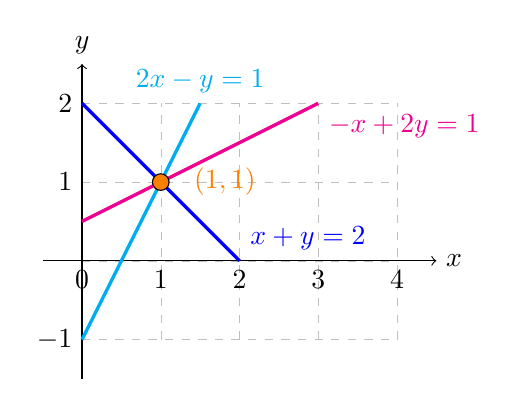
\begin{tikzpicture}
    \draw[step=1,help lines, dashed,lightgray] (0,-1) grid (4,2);
    %draw axis value
    \foreach \x in {0,1,2,3,4}
        {%
            \draw (\x,0) -- (\x,0) node [below] {$\x$};
        }
    \foreach \y in {-1,1,2}
        {%
            \draw (0,\y) -- (0,\y) node [left] {$\y$};
        }
    %draw lines
    \draw [->] (-0.5,0) -- (4.5,0) node[right]{$x$};
    \draw [->] (0,-1.5) -- (0,2.5) node[above]{$y$};
    \draw [-,blue,very thick]  (0,2) -- (2,0) node[above right]{$x+y=2$};
    \draw [-,cyan,very thick]  (0,-1) -- (1.5,2) node[above]{$2x-y=1$};
    \draw [-,magenta,very thick]  (0,0.5) -- (3,2) node[below right]{$-x+2y=1$};
    \draw [fill=orange] (1,1) circle[radius=3pt] node[right,orange]{$\hspace{3mm}(1,1)$};
\end{tikzpicture}
\captionof{figure}{{\footnotesize solutions are too many}}
\label{fig:linear-system-and-subspaces-d2}
